\part{Week 4}
\chapter{Distance measures for quantum information}
We'll try to quantify how two information items are similar, how information is preserved over a process etc. For this, we'll define two classes \textit{distance measures}, \textit{static distance} which is how close two quantum states are, and \textit{dynamic distance} which is how well information is stored over a process. We'll define static distance properly first then build up dynamic distnance with it. Two widely used distance measures currently are \textit{trace distance} and \textit{fidelity}.

\section{Distance measures for classical information}
\textit{Hamming distance} is defined to quantify distance between two bit strings. It's equal to number of mismatching bits (eg. $\text{Hamming}(1011,0010)=2$. But this relies on labelling which we don't have in our Hilbert space arena of quantum mechanics.

We can define a classical information source as a random variable over the set of possible outcomes. So we know the probabilities of getting a given output. In this notion, we can compare two information sources with same index set using a distance measure known as \textit{trace distance}, defined as
\begin{equation}
    D(p_x, q_x) = \frac{1}{2}\sum_x |p_x-q_x|
\end{equation}
where $\{ p_x \}$ and $\{ q_x \}$ are probability distributions of both sources. This is also known as the \textit{$L_1$ distance} or \textit{Kolmogorov distance}. Trace because we use trace when we define this for quantum systems. This is a metric since it satisfies symmetricity ($D(x,y)=D(y,x)$) and triangle inequality ($D(x,y)\leq D(x,z)+D(y,z)$.

\textit{Fidelity}, a second measure is described by
\begin{equation}
    F(p_x, q_x) = \sum \sqrt{p_xq_x}
\end{equation}
This is not a metric as shown by it's physical interpretation in figure \ref{fig:fidelity-distance}.
\begin{figure}
    \centering
    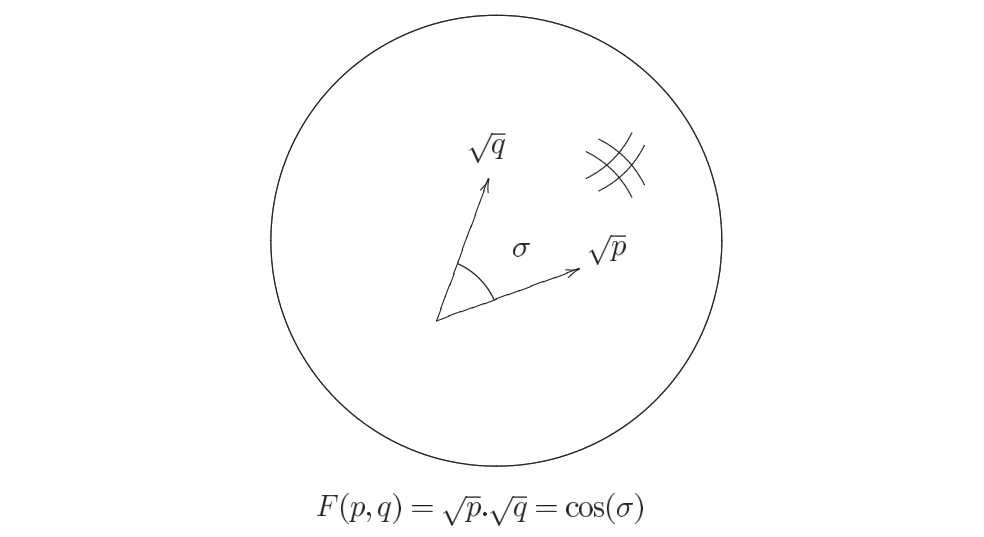
\includegraphics[width=0.9\textwidth]{images/fidelity_distance.png}
    \caption{$F(p_x,q_x)$ can be seen as dot product between $\sqrt{p}$ and $\sqrt{q}$, each of them lie on a unit sphere since $\sum_x \left( \sqrt{p_x} \right)^2 = 1$ and $\sum_x \left( \sqrt{q_x} \right)^2 = 1$}
    \label{fig:fidelity-distance}
\end{figure}

A physically motivated operational meaning for trace distance which can be proved is,
\begin{equation}
    D(p_x, q_x) = \max_S |p(S) - q(S)| = \max_S \left| \sum_{x\in S} p_x - \sum_{x \in S} q_x \right|
\end{equation}
which is maximum over all subsets over index set. This makes sense because $S$ represents an event which produces maximum difference in outputs. It can also be shown that the absolute value is redundant, i.e
\begin{equation}
    D(p_x, q_x) = \max_S \left( \sum_{x\in S} p_x - \sum_{x \in S} q_x\right)
\end{equation}
Trace distance and fidelity are static distance measures.

For \textit{dynamic measure} of distance, suppose a random variable $X$ is passed through a noise channel to produce $Y$ shown by Markov process $X\longrightarrow Y$, a dynamic measure showing how much information is preserved is $p(X\neq Y)$. This can be done using trace distance, for which let's construct a copy $\Tilde{X}$ of $X$ which is also a random variable. Now $X$ is passed through the channel, leaving output $Y$. The closeness between initial perfectly correlated pair $(\Tilde{X}, X)$ and the pair $(\Tilde{X}, Y)$ can be shown to be
\begin{equation}
    D((\Tilde{X},X), (X, Y)) = p(X\neq Y)
\end{equation}
This thing we did to calculate $p(X\neq Y)$ is unique to classical mechanics. We can't \textit{directly} calculate quantum analogue of $p(X\neq Y)$ if $X$ and $Y$ exist at different times. We use quantum entanglement to define dynamic measure similar to the construction shown above. 
\begin{figure}[H]
    \centering
    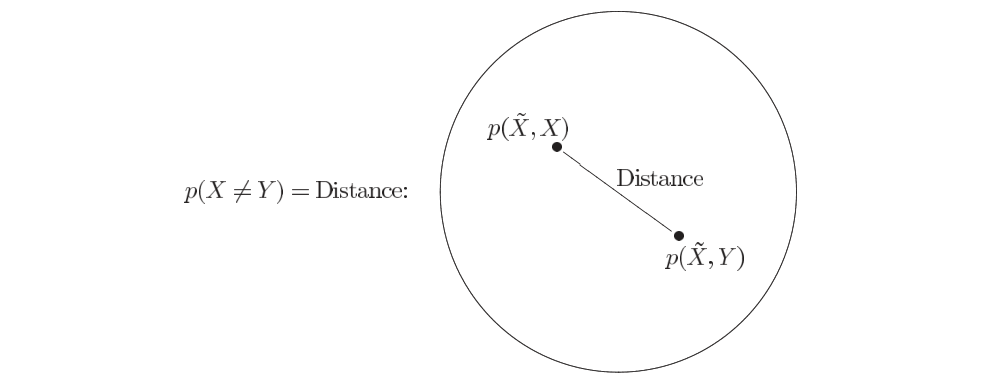
\includegraphics[width=0.8\textwidth]{images/dynamic_measure.png}
    \caption{The probability of an error in the channel is equal to the trace distance between the probability distributions for $( \Tilde{X}, X)$ and $( \Tilde{X}, Y )$.}
    \label{fig:enter-label}
\end{figure}

\section{How close are two quantum states}
We'll see quantum generalizations of trace distance and fidelity.
\subsection{Trace distance}
\textit{Trace distance} between two quantum states $\rho$ and $\sigma$ is defined as
\begin{equation}
    D(\rho, \sigma) = \frac{1}{2}\text{tr} |\rho-\sigma|
\end{equation}
here $|A|=\sqrt{A^\dag A}$. If $\rho$ and $\sigma$ commute (matrix multiplication), this reduces to classical trace distance. Suppose $\rho$ and $\sigma$ commute, then
\begin{align}
    \rho = \sum_i r_i \op{i};
    \ \ \ 
    \sigma = \sum_i s_i \op{i}
\end{align}
for orthogonal basis $\ket{i}$. Then trace distance becomes
\begin{align}
    D(\rho, \sigma) &= \frac{1}{2}\text{tr}|\rho-\sigma| \\
    &= \frac{1}{2}\text{tr}|(r_i-s_i)\op{i}| \\
    &= D(r_i, s_i)
\end{align}
For qubits in Bloch sphere representation, it becomes nicer. Let
\begin{align}
    \rho = \frac{1+\Vec{r}\Vec{\sigma}}{2};
    \ \ \ 
    \sigma = \frac{1+\Vec{s}\Vec{\sigma}}{2}
\end{align}
then trace distance between $\rho$ and $\sigma$ is
\begin{align}
    D(\rho, \sigma) = \frac{|\Vec{r}-\Vec{s}|}{2}
\end{align}
using the fact that $(\Vec{r}-\Vec{s})\cdot \Vec{\sigma}$ has eigen values $\pm |\Vec{r}-\Vec{s}|$. It can be shown that

\begin{equation}
    D(\rho, \sigma) = \max_P \tr{P(\rho-\sigma)}
\end{equation}
where maximum is over all positive operators $P$, $P\leq I$.

\begin{theorem}
    Let $\{ E_m \}$ me a POVM, with $p_m \equiv \tr{\rho E_m}$ and $q_m \equiv \tr{\sigma E_m}$ be the probability of getting output labelled by $m$. Then
    \begin{equation}
        D(\rho, \sigma) = \max_{\{ E_m \} } D(p_m, q_m)
    \end{equation}
    where maximization is over all POVMs $\{ E_m \}$.
\end{theorem}
It can be shown that this trace distance is also a metric. Here goes another nice theorem

\begin{theorem}
    Suppose $\mathcal{E}$ is a trace preserving quantum operation. Let $\rho$, $\sigma$ be density operators. Then
    \begin{equation}
        D(\E{\rho}, \E{\sigma}) \leq D(\rho, \sigma)
    \end{equation}
\end{theorem}
Thus there exists no physical processes which increases distance between two states.
\begin{figure}[H]
    \centering
    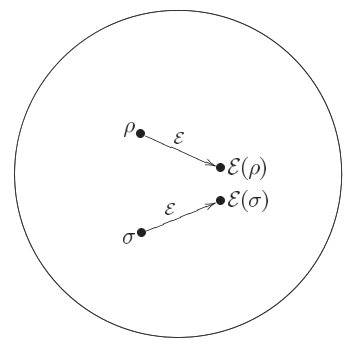
\includegraphics[width=0.4\textwidth]{images/contraction_due_to_operation.png}
    \caption{Trace-preserving quantum operations cause a contraction on the space of density operators.}
    \label{fig:enter-label}
\end{figure}

It can also be showed that
\begin{align}
    D(\rho^A, \sigma^A) \leq D(\rho^{AB}, \sigma^{AB})
\end{align}
intuitively, it's  like things are less differentiable if corresponding parts of them are covered.

\begin{theorem}[\textbf{Strong convexity of trace distance}]
    Let $\{ p_i \}$ and $\{ q_i \}$ be two probability distributions over the same index set, and $\rho_i$, $\sigma_i$ be density operators, also with indices from same index set, then
    \begin{equation}
        D\left( \sum_i p_i\rho_i, \sum_i q_i\sigma_i \right)
        \leq
        D(p_i, q_i) +
        \sum_i p_i D(\rho_i, \sigma_i)
    \end{equation}
    where $D(p_i, q_i)$ is the trace distance between the probability distributions $p_i$ and $q_i$.
\end{theorem}
using this we can show convexity properties of trace distance,
\begin{equation}
    D\left( \sum_i p_i\rho_i , \sigma \right)
    \leq
    \sum_i p_iD(\rho_i, \sigma)
\end{equation}
Also, any trace-preserving quantum operation $\mathcal{E}$ has a fixed point $\rho$ such that $\E{\rho} = \rho$.

\subsection{Fidelity}
\textit{Fidelity} is not a metric on  density operators but does give rise to a useful metric. Fidelity of state $\rho$ and $\sigma$ is defined as
\begin{equation}
    F(\rho, \sigma) \equiv \text{tr}\sqrt{\rho^{1/2}\sigma \rho^{1/2}}
\end{equation}
when $\rho$ and $\sigma$ commute, then
\begin{align}
    \rho = \sum_i p_i\op{i};
    \ \ \ \ 
    \sigma = \sum_i s_i\op{i}
\end{align}
for orthoonormal basis $\ket{i}$, we see that
\begin{align}
    F(\rho, \sigma) &= \text{tr}\sqrt{\sum_i r_is_i\op{i}} \\
    &= \text{tr}\left( \sum_i\sqrt{r_is_i}\op{i} \right) \\
    &= \sum_i \sqrt{r_is_i} \\
    &= F(r_i, s_i)
\end{align}
thus, when $\rho$ and $\sigma$ commute, quantum fidelity reduces to classical fidelity between eigenvalue distributions $r_i$, $s_i$ of $\rho$, $\sigma$ respectively. Also the fidelity between a pure state $\qv$ and an arbitrary state $\rho$ is
\begin{align}
    F(\qv, \rho) &= \text{tr}\sqrt{\bra{\psi}\rho\qv \qv \bra{\psi}} \\
    &= \sqrt{\bra{\psi}\rho\qv}
\end{align}
i.e fidelity is square root of overlap between $\qv$ and $\rho$.

There's no similar Bloch sphere representation for fidelity but it does satisfy similar properties like \textit{invariance under unitary transformation} i.e
\begin{align}
    F(U\rho U^\dag, U\sigma U^\dag) = F(\rho, \sigma)
\end{align}

\begin{theorem}[\textbf{Uhlmann's theorem}]
    Suppose $\rho$, $\sigma$ be states of a system $Q$, Let $R$ be a copy of $Q$. Then
    \begin{equation}
        F(\rho, \sigma) = \max_{\qv, \ket{\varphi}} \left| \braket{\psi | \varphi} \right|
    \end{equation}
    where the maximization is over all purifications $\qv$ of $\rho$ and $\ket{\varphi}$ of $\sigma$.
\end{theorem}

\begin{lemma}
    Let $A$ be any operator, $U$ be unitary. Then
    \begin{equation}
        |\tr{AU}| \leq |\tr{A}|
    \end{equation}
    equality is when $U=V^\dag$ when $A=|A|V$ is polar decomposition of $A$.
\end{lemma}
By Uhlmann's formula it can be shown that fidelity is \textit{symmetric} in its inputs i.e $F(\rho, \sigma) = F(\sigma, \rho)$ and also that it's bound, $0 \leq F(\rho, \sigma) \leq 1$. Also $\rho=\sigma \implies F(\rho, \sigma)=1$ else it's less than 1.